\setchapterimage[2cm]{../images/header-stx.jpg}
%\setchapterpreamble[u]{\margintoc}
\chapter{Sunflower-saxitoxin complexes}
\labch{stx}

\begin{marginfigure}
    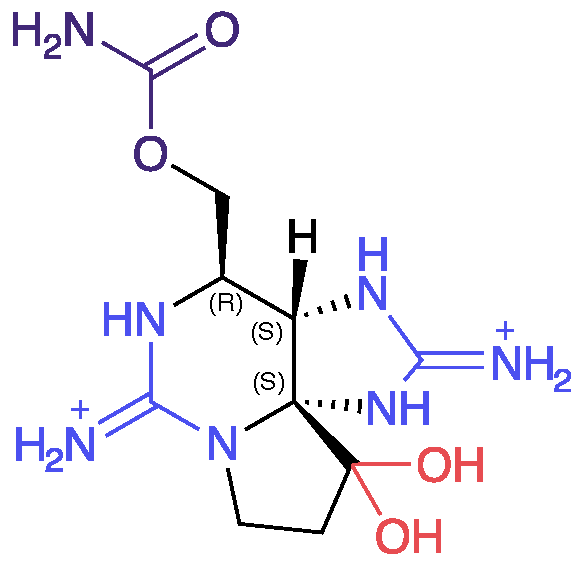
\includegraphics{stx-structure}
    \caption[Structure of STX]{Structure of STX}
    \labfig{stx-structure}
\end{marginfigure}

Having obtained a general characterization of the sunflower-type molecules, it's time to get back to the problem at hand and start looking into how they can be applied.

Let's reintroduce the molecule that motivated this whole study: saxitoxin (STX).
For the purposes of this study, the STX structure features two guanidinium moieties (which are protonated due to the simulation of acidic conditions), two hydroxyl, and one carbamate group as it can be seen in \reffig{stx-structure}.

\blindtext

\section{Spectroscopic study of lone STX}

\blindtext[3]

\section{Study of adsorption}
\blindtext
\subsection{Sampling and optimization}
\blindtext
\subsection{Maxwell-Boltzmann statistics}
\blindtext
\subsection{Basis Set Superposition Error correction}
\blindtext

\section{Study of non-covalent interactions}
\blindtext

\section{Study of UV behavior}
\blindtext
\subsection{General UV spectroscopy}
\blindtext
\subsection{Charge transfer analysis}
\blindtext

\section{Resonance Raman}
\blindtext
\subsection{Generation and comparison of spectra}
\blindtext
\subsection{Combined resonance graphs}
\blindtext
\subsection{Final selection}
\blindtext
